% questions.tex —— 2011 年·全国大纲卷·理科 · 题目内容片段（无答案）
% 由 tools/generate_projects.py 依来源总账自 2011/2011_数学真题_全国大纲理_试题.md 生成，勿手改（改源 MD 后重跑）


\gkpart{数学}

\begin{gktip}
\textbf{来源说明}：本题面依据固定源 PDF 两页 A3 题面逐题转录，原卷印刷页码 655–656。固定源不附答案，答案和解析均由本库独立复算。

\textbf{图形说明}：第 19、21 题的原卷立体图或坐标图重绘为 TikZ/PGFPlots 矢量图。图形标记所指的 PNG 不随仓库保存。
\end{gktip}

\gkpart{一、选择题}

\begin{question}
\gkti{1}复数 $z=1+i$，$\overline z$ 为 $z$ 的共轭复数，则 $z\overline z-z-1=$\mbox{（　　）}

（A）$-2i$\quad（B）$-i$\quad（C）$i$\quad（D）$2i$

\end{question}
\begin{question}
\gkti{2}函数 $y=2\sqrt{x}$（$x\geq0$）的反函数为\mbox{（　　）}

（A）$y=\dfrac{x^2}{4}$（$x\in\mathbb R$）\quad（B）$y=\dfrac{x^2}{4}$（$x\geq0$）

（C）$y=4x^2$（$x\in\mathbb R$）\quad（D）$y=4x^2$（$x\geq0$）

\end{question}
\begin{question}
\gkti{3}下面四个条件中，使 $a>b$ 成立的充分而不必要的条件是\mbox{（　　）}

（A）$a>b+1$\quad（B）$a>b-1$\quad（C）$a^2>b^2$\quad（D）$a^3>b^3$

\end{question}
\begin{question}
\gkti{4}设 $S_n$ 为等差数列 $\{a_n\}$ 的前 $n$ 项和，若 $a_1=1$，公差 $d=2$，$S_{k+2}-S_k=24$，则 $k=$\mbox{（　　）}

（A）$8$\quad（B）$7$\quad（C）$6$\quad（D）$5$

\end{question}
\begin{question}
\gkti{5}设函数 $f(x)=\cos\omega x$（$\omega>0$），将 $y=f(x)$ 的图象向右平移 $\dfrac\pi3$ 个单位长度后，所得的图象与原图象重合，则 $\omega$ 的最小值等于\mbox{（　　）}

（A）$\dfrac13$\quad（B）$3$\quad（C）$6$\quad（D）$9$

\end{question}
\begin{question}
\gkti{6}已知直二面角 $\alpha-l-\beta$，点 $A\in\alpha$，$AC\perp l$，$C$ 为垂足，点 $B\in\beta$，$BD\perp l$，$D$ 为垂足。若 $AB=2$，$AC=BD=1$，则 $CD=$\mbox{（　　）}

（A）$\dfrac{\sqrt2}{3}$\quad（B）$\dfrac{\sqrt3}{3}$\quad（C）$\dfrac{\sqrt6}{3}$\quad（D）$1$

\end{question}
\begin{question}
\gkti{7}某同学有同样的画册 $2$ 本、同样的集邮册 $3$ 本，从中取出 $4$ 本赠送给 $4$ 位朋友，每位朋友 $1$ 本，则不同的赠送方法共有\mbox{（　　）}

（A）$4$ 种\quad（B）$10$ 种\quad（C）$18$ 种\quad（D）$20$ 种

\end{question}
\begin{question}
\gkti{8}曲线 $y=e^{-2x}+1$ 在点 $(0,2)$ 处的切线与直线 $y=0$ 和 $y=x$ 围成的三角形的面积为\mbox{（　　）}

（A）$\dfrac13$\quad（B）$\dfrac12$\quad（C）$\dfrac23$\quad（D）$1$

\end{question}
\begin{question}
\gkti{9}设 $f(x)$ 是周期为 $2$ 的奇函数，当 $0\leq x\leq1$ 时，$f(x)=2x(1-x)$，则 $f\left(-\dfrac52\right)=$\mbox{（　　）}

（A）$-\dfrac12$\quad（B）$-\dfrac14$\quad（C）$\dfrac14$\quad（D）$\dfrac12$

\end{question}
\begin{question}
\gkti{10}已知抛物线 $C:y^2=4x$ 的焦点为 $F$，直线 $y=2x-4$ 与 $C$ 交于 $A\text{、}B$ 两点，则 $\cos\angle AFB=$\mbox{（　　）}

（A）$\dfrac45$\quad（B）$\dfrac35$\quad（C）$-\dfrac35$\quad（D）$-\dfrac45$

\end{question}
\begin{question}
\gkti{11}已知平面 $\alpha$ 截一球面得圆 $M$，过圆心 $M$ 且与 $\alpha$ 成 $60^\circ$ 二面角的平面 $\beta$ 截该球面得圆 $N$。若该球面的半径为 $4$，圆 $M$ 的面积为 $4\pi$，则圆 $N$ 的面积为\mbox{（　　）}

（A）$7\pi$\quad（B）$9\pi$\quad（C）$11\pi$\quad（D）$13\pi$

\end{question}
\begin{question}
\gkti{12}设向量 $\boldsymbol a\text{、}\boldsymbol b\text{、}\boldsymbol c$ 满足 $|\boldsymbol a|=|\boldsymbol b|=1$，$\boldsymbol a\cdot\boldsymbol b=-\dfrac12$，$\langle\boldsymbol a-\boldsymbol c,\boldsymbol b-\boldsymbol c\rangle=60^\circ$，则 $|\boldsymbol c|$ 的最大值等于\mbox{（　　）}

（A）$2$\quad（B）$\sqrt3$\quad（C）$\sqrt2$\quad（D）$1$

\end{question}
\gkpart{二、填空题}

\begin{question}
\gkti{13}$(1-\sqrt{x})^{20}$ 的二项展开式中，$x$ 的系数与 $x^9$ 的系数之差为\gkblank{}。

\end{question}
\begin{question}
\gkti{14}已知 $\alpha\in\left(\dfrac\pi2,\pi\right)$，$\sin\alpha=\dfrac{\sqrt5}{5}$，则 $\tan2\alpha=$\gkblank{}。

\end{question}
\begin{question}
\gkti{15}已知 $F_1\text{、}F_2$ 分别为双曲线 $C:\dfrac{x^2}{9}-\dfrac{y^2}{27}=1$ 的左、右焦点，点 $A\in C$，点 $M$ 的坐标为 $(2,0)$，$AM$ 为 $\angle F_1AF_2$ 的平分线，则 $|AF_2|=$\gkblank{}。

\end{question}
\begin{question}
\gkti{16}已知点 $E\text{、}F$ 分别在正方体 $ABCD-A_1B_1C_1D_1$ 的棱 $BB_1\text{、}CC_1$ 上，且 $B_1E=2EB$，$CF=2FC_1$，则面 $AEF$ 与面 $ABC$ 所成的二面角的正切值等于\gkblank{}。

\end{question}
\gkpart{三、解答题}

\begin{question}
\gkti{17}$\triangle ABC$ 的内角 $A\text{、}B\text{、}C$ 的对边分别为 $a\text{、}b\text{、}c$。已知 $A-C=90^\circ$，$a+c=2b$，求 $C$。

\end{question}
\begin{question}
\gkti{18}根据以往统计资料，某地车主购买甲种保险的概率为 $0.5$，购买乙种保险但不购买甲种保险的概率为 $0.3$。设各车主购买保险相互独立。

（1） 求该地 $1$ 位车主至少购买甲、乙两种保险中的 $1$ 种的概率；

（2） $X$ 表示该地的 $100$ 位车主中，甲、乙两种保险都不购买的车主数。求 $X$ 的期望。

\Needspace{0.4\textheight}
\end{question}
\begin{question}
\gkti{19}如图，四棱锥 $S-ABCD$ 中，$AB\parallel CD$，$BC\perp CD$，侧面 $SAB$ 为等边三角形。$AB=BC=2$，$CD=SD=1$。
\nopagebreak[4]
\begin{center}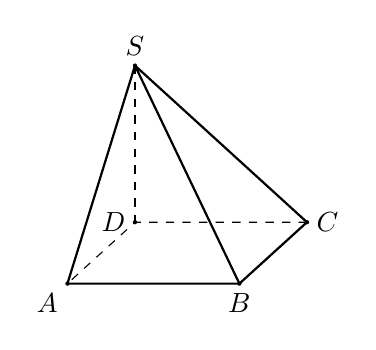
\begin{tikzpicture}[scale=.78,>=stealth]
\coordinate (A) at (0,0);
\coordinate (B) at (2.8,0);
\coordinate (C) at (3.9,1.0);
\coordinate (D) at (1.1,1.0);
\coordinate (S) at (1.1,3.55);
\draw[thick] (A)--(B)--(C);
\draw[dashed] (C)--(D)--(A);
\draw[thick] (S)--(A) (S)--(B) (S)--(C);
\draw[dashed] (S)--(D);
\fill (A) circle (1pt) node[below left] {$A$};
\fill (B) circle (1pt) node[below] {$B$};
\fill (C) circle (1pt) node[right] {$C$};
\fill (D) circle (1pt) node[left] {$D$};
\fill (S) circle (1pt) node[above] {$S$};
\end{tikzpicture}
\end{center}
\nopagebreak[4]
（1） 证明：$SD\perp$ 平面 $SAB$；

（2） 求 $AB$ 与平面 $SBC$ 所成角的正弦值。

\end{question}
\begin{question}
\gkti{20}设数列 $\{a_n\}$ 满足 $a_1=0$ 且

\nopagebreak[4]
\[
\frac{1}{1-a_{n+1}}-\frac{1}{1-a_n}=1.
\]

（1） 求 $\{a_n\}$ 的通项公式；

（2） 设 $b_n=\dfrac{1-\sqrt{a_{n+1}}}{\sqrt n}$，记 $S_n=\displaystyle\sum_{k=1}^n b_k$，证明：$S_n<1$。

\Needspace{0.4\textheight}
\end{question}
\begin{question}
\gkti{21}已知 $O$ 为坐标原点，$F$ 为椭圆 $C:x^2+\dfrac{y^2}{2}=1$ 在 $y$ 轴正半轴上的焦点，过 $F$ 且斜率为 $-\sqrt2$ 的直线 $l$ 与 $C$ 交于 $A\text{、}B$ 两点，点 $P$ 满足

\nopagebreak[4]
\[
\overrightarrow{OA}+\overrightarrow{OB}+\overrightarrow{OP}=\boldsymbol0.
\]
\nopagebreak[4]
\begin{center}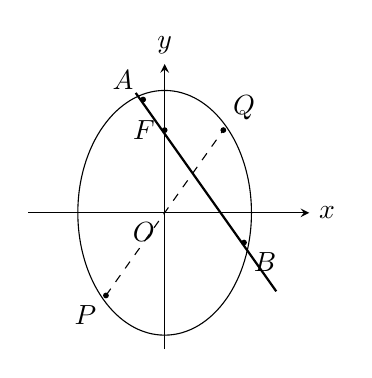
\begin{tikzpicture}[>=stealth,scale=1.05]
\draw[->] (-1.65,0)--(1.75,0) node[right] {$x$};
\draw[->] (0,-1.65)--(0,1.8) node[above] {$y$};
\draw (0,0) ellipse [x radius=1.05,y radius=1.48];
\draw[thick] (-.35,1.45)--(1.35,-.95);
\fill (-.26,1.37) circle (1pt) node[above left] {$A$};
\fill (.96,-.36) circle (1pt) node[below right] {$B$};
\fill (0,1) circle (1pt) node[left] {$F$};
\fill (-.71,-1) circle (1pt) node[below left] {$P$};
\fill (.71,1) circle (1pt) node[above right] {$Q$};
\draw[dashed] (-.71,-1)--(.71,1);
\node[below left] at (0,0) {$O$};
\end{tikzpicture}
\end{center}
\nopagebreak[4]
（1） 证明：点 $P$ 在 $C$ 上；

（2） 设点 $P$ 关于点 $O$ 的对称点为 $Q$，证明：$A\text{、}P\text{、}B\text{、}Q$ 四点在同一圆上。

\end{question}
\begin{question}
\gkti{22}（1） 设函数 $f(x)=\ln(1+x)-\dfrac{2x}{x+2}$，证明：当 $x>0$ 时，$f(x)>0$；

\Needspace{5\baselineskip}
（2） 从编号 $1$ 到 $100$ 的 $100$ 张卡片中每次随机抽取一张，然后放回，用这种方式连续抽取 $20$ 次，设抽得的 $20$ 个号码互不相同的概率为 $p$。证明：

\nopagebreak[4]
\[
p<\left(\frac9{10}\right)^{19}<\frac1{e^2}.
\]

\end{question}